% Options for packages loaded elsewhere
\PassOptionsToPackage{unicode}{hyperref}
\PassOptionsToPackage{hyphens}{url}
%
\documentclass[
  a4paper,
]{article}
\usepackage{amsmath,amssymb}
\usepackage{iftex}
\ifPDFTeX
  \usepackage[T1]{fontenc}
  \usepackage[utf8]{inputenc}
  \usepackage{textcomp} % provide euro and other symbols
\else % if luatex or xetex
  \usepackage{unicode-math} % this also loads fontspec
  \defaultfontfeatures{Scale=MatchLowercase}
  \defaultfontfeatures[\rmfamily]{Ligatures=TeX,Scale=1}
\fi
\usepackage{lmodern}
\ifPDFTeX\else
  % xetex/luatex font selection
  \setmainfont[]{Helvetica}
\fi
% Use upquote if available, for straight quotes in verbatim environments
\IfFileExists{upquote.sty}{\usepackage{upquote}}{}
\IfFileExists{microtype.sty}{% use microtype if available
  \usepackage[]{microtype}
  \UseMicrotypeSet[protrusion]{basicmath} % disable protrusion for tt fonts
}{}
\makeatletter
\@ifundefined{KOMAClassName}{% if non-KOMA class
  \IfFileExists{parskip.sty}{%
    \usepackage{parskip}
  }{% else
    \setlength{\parindent}{0pt}
    \setlength{\parskip}{6pt plus 2pt minus 1pt}}
}{% if KOMA class
  \KOMAoptions{parskip=half}}
\makeatother
\usepackage{xcolor}
\usepackage[margin=0.75in]{geometry}
\usepackage{graphicx}
\makeatletter
\def\maxwidth{\ifdim\Gin@nat@width>\linewidth\linewidth\else\Gin@nat@width\fi}
\def\maxheight{\ifdim\Gin@nat@height>\textheight\textheight\else\Gin@nat@height\fi}
\makeatother
% Scale images if necessary, so that they will not overflow the page
% margins by default, and it is still possible to overwrite the defaults
% using explicit options in \includegraphics[width, height, ...]{}
\setkeys{Gin}{width=\maxwidth,height=\maxheight,keepaspectratio}
% Set default figure placement to htbp
\makeatletter
\def\fps@figure{htbp}
\makeatother
\setlength{\emergencystretch}{3em} % prevent overfull lines
\providecommand{\tightlist}{%
  \setlength{\itemsep}{0pt}\setlength{\parskip}{0pt}}
\setcounter{secnumdepth}{-\maxdimen} % remove section numbering
\usepackage{titling}
\pretitle{\begin{flushleft}}
\posttitle{\end{flushleft}}
\usepackage{booktabs}
\usepackage{longtable}
\usepackage{float}
\floatplacement{figure}{H}
\usepackage{colortbl}
\usepackage{pdflscape}
\usepackage{tabu}
\usepackage{makecell}
\usepackage{xcolor}
\usepackage{soul}
\usepackage{caption}
\usepackage[singlelinecheck=false]{caption}
\usepackage[font={small,bf}]{caption}
\usepackage{multirow}
\usepackage{array}
\usepackage{lscape}
\newcommand{\blandscape}{\begin{landscape}}
\newcommand{\elandscape}{\end{landscape}}
\usepackage{booktabs}
\usepackage{longtable}
\usepackage{array}
\usepackage{multirow}
\usepackage{wrapfig}
\usepackage{float}
\usepackage{colortbl}
\usepackage{pdflscape}
\usepackage{tabu}
\usepackage{threeparttable}
\usepackage{threeparttablex}
\usepackage[normalem]{ulem}
\usepackage{makecell}
\usepackage{xcolor}
\ifLuaTeX
  \usepackage{selnolig}  % disable illegal ligatures
\fi
\usepackage{bookmark}
\IfFileExists{xurl.sty}{\usepackage{xurl}}{} % add URL line breaks if available
\urlstyle{same}
\hypersetup{
  hidelinks,
  pdfcreator={LaTeX via pandoc}}

\title{\vspace{-1.5cm} \begin{LARGE} WGS Quality Control Report \end{LARGE}}
\author{}
\date{\vspace{-2.5em}}

\begin{document}
\maketitle

\normalsize Batch Name: 2024-07-28

\normalsize Experiment Name: 24ARS\_SALM2\_LG735

\fontsize{7}{8}
\selectfont
\captionsetup[table]{labelformat=empty}
\renewcommand{\arraystretch}{1.2}

\begin{longtable}[t]{>{\centering\arraybackslash}p{1cm}>{\centering\arraybackslash}p{2cm}>{\centering\arraybackslash}p{1.5cm}>{\centering\arraybackslash}p{5.25cm}>{\centering\arraybackslash}p{5.25cm}}
\toprule
\multicolumn{1}{>{\centering\arraybackslash}p{1cm}}{\cellcolor[HTML]{D4D4D4}{\textbf{Isolate No.}}} & \multicolumn{1}{>{\centering\arraybackslash}p{2cm}}{\cellcolor[HTML]{D4D4D4}{\textbf{Sample ID}}} & \multicolumn{1}{>{\centering\arraybackslash}p{1.5cm}}{\cellcolor[HTML]{D4D4D4}{\textbf{Description}}} & \multicolumn{1}{>{\centering\arraybackslash}p{5.25cm}}{\cellcolor[HTML]{D4D4D4}{\textbf{ARSRL}}} & \multicolumn{1}{>{\centering\arraybackslash}p{5.25cm}}{\cellcolor[HTML]{D4D4D4}{\textbf{WGS}}}\\
\midrule
1 & 24ARS\_BGH0073 & SAL83 & Salmonella species & \cellcolor{white}{Salmonella enterica}\\
2 & 24ARS\_BGH0098 & SAL84 & Salmonella species & \cellcolor{white}{Salmonella enterica subsp. enterica serovar Infantis}\\
3 & 24ARS\_BGH0099 & SAL85 & Salmonella species & \cellcolor{white}{Salmonella enterica subsp. enterica serovar Typhimurium}\\
4 & 24ARS\_BGH0100 & SAL86 & Salmonella species & \cellcolor{white}{Salmonella enterica subsp. enterica serovar Infantis}\\
\cellcolor[HTML]{FFA77F}{5} & \cellcolor[HTML]{FFA77F}{24ARS\_BRH0012} & \cellcolor[HTML]{FFA77F}{SAL87} & \cellcolor[HTML]{FFA77F}{Salmonella species} & \cellcolor[HTML]{FFA77F}{Salmonella enterica subsp. enterica serovar Enteritidis}\\
\addlinespace
6 & 24ARS\_BRH0013 & SAL88 & Salmonella species & \cellcolor{white}{Salmonella enterica subsp. enterica serovar Enteritidis}\\
7 & 24ARS\_BRH0054 & SAL89 & Salmonella species & \cellcolor{white}{Salmonella enterica subsp. enterica serovar Typhimurium}\\
8 & 24ARS\_BRH0068 & SAL90 & Salmonella species & \cellcolor{white}{Salmonella enterica subsp. enterica serovar Typhi}\\
9 & 24ARS\_BRT0028 & SAL91 & Salmonella Typhi & \cellcolor{white}{Salmonella enterica subsp. enterica serovar Typhi}\\
\cellcolor[HTML]{FFA77F}{10} & \cellcolor[HTML]{FFA77F}{24ARS\_BRT0041} & \cellcolor[HTML]{FFA77F}{SAL92} & \cellcolor[HTML]{FFA77F}{Salmonella species} & \cellcolor[HTML]{FFA77F}{Salmonella enterica}\\
\addlinespace
11 & 24ARS\_CMC0007 & SAL93 & Salmonella Typhi & \cellcolor{white}{Salmonella enterica subsp. enterica serovar Typhi}\\
\cellcolor[HTML]{FFA77F}{12} & \cellcolor[HTML]{FFA77F}{24ARS\_CRH0031} & \cellcolor[HTML]{FFA77F}{SAL94} & \cellcolor[HTML]{FFA77F}{Salmonella species} & \cellcolor[HTML]{FFA77F}{Salmonella enterica}\\
\cellcolor[HTML]{FFA77F}{13} & \cellcolor[HTML]{FFA77F}{24ARS\_CRH0049} & \cellcolor[HTML]{FFA77F}{SAL95} & \cellcolor[HTML]{FFA77F}{Salmonella species} & \cellcolor[HTML]{FFA77F}{Salmonella enterica subsp. enterica serovar Typhimurium}\\
14 & 24ARS\_CVM0082 & SAL96 & Salmonella Typhi & \cellcolor{white}{Salmonella enterica subsp. enterica serovar Typhi}\\
15 & 24ARS\_DMC0100 & SAL97 & Salmonella species & \cellcolor{white}{Salmonella enterica subsp. enterica serovar Weltevreden}\\
\addlinespace
16 & 24ARS\_DMC0101 & SAL98 & Salmonella species & \cellcolor{white}{Salmonella enterica subsp. enterica serovar Weltevreden}\\
17 & 24ARS\_DMC0162 & SAL99 & Salmonella species & \cellcolor{white}{Salmonella enterica}\\
18 & 24ARS\_DMC0218 & SAL100 & Salmonella Typhi & \cellcolor{white}{Salmonella enterica subsp. enterica serovar Typhi}\\
19 & 24ARS\_DMC0291 & SAL101 & Salmonella species & \cellcolor{white}{Salmonella enterica}\\
20 & 24ARS\_DMC0292 & SAL102 & Salmonella Typhi & \cellcolor{white}{Salmonella enterica subsp. enterica serovar Typhi}\\
\addlinespace
\cellcolor[HTML]{FFA77F}{21} & \cellcolor[HTML]{FFA77F}{24ARS\_GMH0033} & \cellcolor[HTML]{FFA77F}{SAL103} & \cellcolor[HTML]{FFA77F}{Salmonella species} & \cellcolor[HTML]{FFA77F}{Salmonella enterica}\\
22 & 24ARS\_JLM0046 & SAL104 & Salmonella species & \cellcolor{white}{Salmonella enterica subsp. enterica serovar Infantis}\\
\bottomrule
\end{longtable}

\tiny Legend: \begingroup\fontsize{4}{6}\selectfont

\begin{tabular}{|>{\centering\arraybackslash}p{1cm}|>{\centering\arraybackslash}p{1cm}|>{\centering\arraybackslash}p{1cm}|>{\centering\arraybackslash}p{3cm}|>{\centering\arraybackslash}p{2cm}|}

\cellcolor{white}{PASS} & \cellcolor[HTML]{FFA77F}{WARNING} & \cellcolor[HTML]{FD7979}{FAILURE} & \textcolor{blue}{EXCEEDS THRESHOLD METRIC/S} & \cellcolor{yellow}{NON-CONCORDANT}\\

\end{tabular}
\endgroup{}
\fontsize{7}{8}
\selectfont
\captionsetup[table]{labelformat=empty}
\renewcommand{\arraystretch}{1.2}

\(\\\)

\fontsize{7}{8}
\selectfont
\captionsetup[table]{labelformat=empty}
\renewcommand{\arraystretch}{1.2}

\begin{longtable}[t]{>{\centering\arraybackslash}p{1cm}>{\centering\arraybackslash}p{3cm}>{\centering\arraybackslash}p{2cm}>{\centering\arraybackslash}p{2cm}>{\centering\arraybackslash}p{2cm}>{\centering\arraybackslash}p{2cm}>{\centering\arraybackslash}p{2cm}}
\toprule
\multicolumn{1}{>{\centering\arraybackslash}p{1cm}}{\cellcolor[HTML]{D4D4D4}{\textbf{Isolate No.}}} & \multicolumn{1}{>{\centering\arraybackslash}p{3cm}}{\cellcolor[HTML]{D4D4D4}{\textbf{Sample ID}}} & \multicolumn{1}{>{\centering\arraybackslash}p{2cm}}{\cellcolor[HTML]{D4D4D4}{\textbf{Contamination}}} & \multicolumn{1}{>{\centering\arraybackslash}p{2cm}}{\cellcolor[HTML]{D4D4D4}{\textbf{Contigs}}} & \multicolumn{1}{>{\centering\arraybackslash}p{2cm}}{\cellcolor[HTML]{D4D4D4}{\textbf{GC Percent}}} & \multicolumn{1}{>{\centering\arraybackslash}p{2cm}}{\cellcolor[HTML]{D4D4D4}{\textbf{N50}}} & \multicolumn{1}{>{\centering\arraybackslash}p{2cm}}{\cellcolor[HTML]{D4D4D4}{\textbf{Total Length}}}\\
\midrule
1 & 24ARS\_BGH0073 & \textcolor{black}{0} & \textcolor{black}{47} & 52.09 & \textcolor{black}{291623} & 5020885\\
2 & 24ARS\_BGH0098 & \textcolor{black}{0} & \textcolor{black}{55} & 52.14 & \textcolor{black}{245434} & 4977405\\
3 & 24ARS\_BGH0099 & \textcolor{black}{0} & \textcolor{black}{38} & 52.17 & \textcolor{black}{376619} & 4913046\\
4 & 24ARS\_BGH0100 & \textcolor{black}{0} & \textcolor{black}{58} & 52.14 & \textcolor{black}{194191} & 4975128\\
\cellcolor[HTML]{FFA77F}{5} & \cellcolor[HTML]{FFA77F}{* 24ARS\_BRH0012} & \cellcolor[HTML]{FFA77F}{\textcolor{black}{0}} & \cellcolor[HTML]{FFA77F}{\textcolor{black}{27}} & \cellcolor[HTML]{FFA77F}{52.03} & \cellcolor[HTML]{FFA77F}{\textcolor{black}{489959}} & \cellcolor[HTML]{FFA77F}{4771132}\\
\addlinespace
6 & 24ARS\_BRH0013 & \textcolor{black}{0} & \textcolor{black}{25} & 52.13 & \textcolor{black}{490385} & 4702229\\
7 & 24ARS\_BRH0054 & \textcolor{black}{0} & \textcolor{black}{61} & 52.12 & \textcolor{black}{263338} & 4950993\\
8 & 24ARS\_BRH0068 & \textcolor{black}{0} & \textcolor{black}{58} & 52.07 & \textcolor{black}{204318} & 4736095\\
9 & 24ARS\_BRT0028 & \textcolor{black}{0} & \textcolor{black}{54} & 52.08 & \textcolor{black}{204323} & 4707276\\
\cellcolor[HTML]{FFA77F}{10} & \cellcolor[HTML]{FFA77F}{* 24ARS\_BRT0041} & \cellcolor[HTML]{FFA77F}{\textcolor{black}{0}} & \cellcolor[HTML]{FFA77F}{\textcolor{black}{22}} & \cellcolor[HTML]{FFA77F}{52.10} & \cellcolor[HTML]{FFA77F}{\textcolor{black}{490374}} & \cellcolor[HTML]{FFA77F}{4721282}\\
\addlinespace
11 & 24ARS\_CMC0007 & \textcolor{black}{0} & \textcolor{black}{58} & 52.09 & \textcolor{black}{153660} & 4701851\\
\cellcolor[HTML]{FFA77F}{12} & \cellcolor[HTML]{FFA77F}{* 24ARS\_CRH0031} & \cellcolor[HTML]{FFA77F}{\textcolor{black}{0}} & \cellcolor[HTML]{FFA77F}{\textcolor{black}{16}} & \cellcolor[HTML]{FFA77F}{52.14} & \cellcolor[HTML]{FFA77F}{\textcolor{black}{697691}} & \cellcolor[HTML]{FFA77F}{4525268}\\
\cellcolor[HTML]{FFA77F}{13} & \cellcolor[HTML]{FFA77F}{* 24ARS\_CRH0049} & \cellcolor[HTML]{FFA77F}{\textcolor{black}{0}} & \cellcolor[HTML]{FFA77F}{\textcolor{black}{38}} & \cellcolor[HTML]{FFA77F}{52.12} & \cellcolor[HTML]{FFA77F}{\textcolor{black}{418650}} & \cellcolor[HTML]{FFA77F}{4707180}\\
14 & 24ARS\_CVM0082 & \textcolor{black}{0} & \textcolor{black}{55} & 52.10 & \textcolor{black}{204322} & 4699960\\
15 & 24ARS\_DMC0100 & \textcolor{black}{0} & \textcolor{black}{89} & 52.04 & \textcolor{black}{219196} & 5135005\\
\addlinespace
16 & 24ARS\_DMC0101 & \textcolor{black}{0} & \textcolor{black}{91} & 52.07 & \textcolor{black}{221808} & 5031480\\
17 & 24ARS\_DMC0162 & \textcolor{black}{0} & \textcolor{black}{52} & 51.32 & \textcolor{black}{403711} & 5081038\\
18 & 24ARS\_DMC0218 & \textcolor{black}{0} & \textcolor{black}{57} & 52.08 & \textcolor{black}{172569} & 4701935\\
19 & 24ARS\_DMC0291 & \textcolor{black}{0} & \textcolor{black}{57} & 52.15 & \textcolor{black}{319335} & 4906095\\
20 & 24ARS\_DMC0292 & \textcolor{black}{0} & \textcolor{black}{58} & 52.08 & \textcolor{black}{161697} & 4733558\\
\addlinespace
\cellcolor[HTML]{FFA77F}{21} & \cellcolor[HTML]{FFA77F}{* 24ARS\_GMH0033} & \cellcolor[HTML]{FFA77F}{\textcolor{black}{0}} & \cellcolor[HTML]{FFA77F}{\textcolor{black}{25}} & \cellcolor[HTML]{FFA77F}{52.07} & \cellcolor[HTML]{FFA77F}{\textcolor{black}{490238}} & \cellcolor[HTML]{FFA77F}{4752483}\\
22 & 24ARS\_JLM0046 & \textcolor{black}{0} & \textcolor{black}{61} & 52.13 & \textcolor{black}{204159} & 4985784\\
\bottomrule
\end{longtable}

\tiny Legend: \begingroup\fontsize{4}{6}\selectfont

\begin{tabular}{|>{\centering\arraybackslash}p{1cm}|>{\centering\arraybackslash}p{1cm}|>{\centering\arraybackslash}p{1cm}|>{\centering\arraybackslash}p{2.5cm}|>{\centering\arraybackslash}p{8cm}|}

\cellcolor{white}{PASS} & \cellcolor[HTML]{FFA77F}{WARNING} & \cellcolor[HTML]{FD7979}{FAILURE} & \textcolor{blue}{EXCEEDS THRESHOLD METRIC/S} & *Isolates were tagged with warning due to uncertain results of species identification using bactinspector.\\

\end{tabular}
\endgroup{}

\fontsize{7}{8}
\selectfont
\captionsetup[table]{labelformat=empty}
\renewcommand{\arraystretch}{1.2}

\begin{longtable}[t]{>{\centering\arraybackslash}p{2cm}>{\raggedright\arraybackslash}p{3cm}>{\centering\arraybackslash}p{11cm}}
\toprule
\multicolumn{3}{l}{\textbf{With Warning/s}} \\
\cmidrule(l{3pt}r{3pt}){1-3}
\multicolumn{1}{>{\centering\arraybackslash}p{2cm}}{\cellcolor[HTML]{D4D4D4}{\textbf{Isolate No.}}} & \multicolumn{1}{>{\centering\arraybackslash}p{3cm}}{\cellcolor[HTML]{D4D4D4}{\textbf{Sample ID}}} & \multicolumn{1}{>{\centering\arraybackslash}p{11cm}}{\cellcolor[HTML]{D4D4D4}{\textbf{Value with warning/s}}}\\
\midrule
\cellcolor{gray!10}{5} & \cellcolor{gray!10}{24ARS\_BRH0012} & \cellcolor{gray!10}{fastqc.1.Per.sequence.GC.content.metric\_value, fastqc.1.Sequence.Length.Distribution.metric\_value, fastqc.2.Per.sequence.GC.content.metric\_value, fastqc.2.Sequence.Length.Distribution.metric\_value}\\
10 & 24ARS\_BRT0041 & fastqc.1.Per.sequence.GC.content.metric\_value, fastqc.1.Sequence.Length.Distribution.metric\_value, fastqc.2.Per.sequence.GC.content.metric\_value, fastqc.2.Sequence.Length.Distribution.metric\_value\\
\cellcolor{gray!10}{12} & \cellcolor{gray!10}{24ARS\_CRH0031} & \cellcolor{gray!10}{fastqc.1.Per.sequence.GC.content.metric\_value, fastqc.1.Sequence.Length.Distribution.metric\_value, fastqc.2.Per.sequence.GC.content.metric\_value, fastqc.2.Sequence.Length.Distribution.metric\_value}\\
13 & 24ARS\_CRH0049 & fastqc.1.Per.sequence.GC.content.metric\_value, fastqc.1.Sequence.Length.Distribution.metric\_value, fastqc.2.Per.sequence.GC.content.metric\_value, fastqc.2.Sequence.Length.Distribution.metric\_value\\
\cellcolor{gray!10}{21} & \cellcolor{gray!10}{24ARS\_GMH0033} & \cellcolor{gray!10}{fastqc.1.Per.sequence.GC.content.metric\_value, fastqc.1.Sequence.Length.Distribution.metric\_value, fastqc.2.Per.sequence.GC.content.metric\_value, fastqc.2.Sequence.Length.Distribution.metric\_value}\\
\bottomrule
\end{longtable}

\begin{longtable}[l]{>{\centering\arraybackslash}p{3cm}>{\centering\arraybackslash}p{12cm}}
\toprule
\multicolumn{2}{l}{\textbf{List of samples above/below QC threshold metrics}} \\
\cmidrule(l{3pt}r{3pt}){1-2}
\cellcolor[HTML]{D4D4D4}{\textbf{Sample ID}} & \cellcolor[HTML]{D4D4D4}{\textbf{Remarks}}\\
\midrule
 & No QC failures found.\\
\bottomrule
\end{longtable}

\fontsize{7}{8}
\selectfont
\captionsetup[table]{labelformat=empty}
\renewcommand{\arraystretch}{1.2}

\begin{longtable}[l]{>{\raggedright\arraybackslash}p{8cm}c}
\toprule
\cellcolor[HTML]{D4D4D4}{\textbf{WGS\_ID}} & \cellcolor[HTML]{D4D4D4}{\textbf{Number}}\\
\midrule
Salmonella enterica & 6\\
Salmonella enterica subsp. enterica serovar Typhi & 6\\
Salmonella enterica subsp. enterica serovar Infantis & 3\\
Salmonella enterica subsp. enterica serovar Typhimurium & 3\\
Salmonella enterica subsp. enterica serovar Enteritidis & 2\\
\addlinespace
Salmonella enterica subsp. enterica serovar Weltevreden & 2\\
\bottomrule
\end{longtable}

\begin{itemize}
\item
  \(\color{red}6\) distinct species were identified among
  \(\color{red}22\) isolates.
\item
  \(\color{red}77.27\) \% (n=17) of the isolates passed the QC, while
  \(\color{red}22.73\) \% (n=5) were tagged with warning.
\item
  Concordance between ARSRL and WGS species report was
  \(\color{red}100.00\) \%. \(\\\)
\end{itemize}

\subsubsection{GRAPHS}\label{graphs}

\fontsize{7}{8}
\selectfont
\captionsetup[table]{labelformat=empty}
\renewcommand{\arraystretch}{1.2}

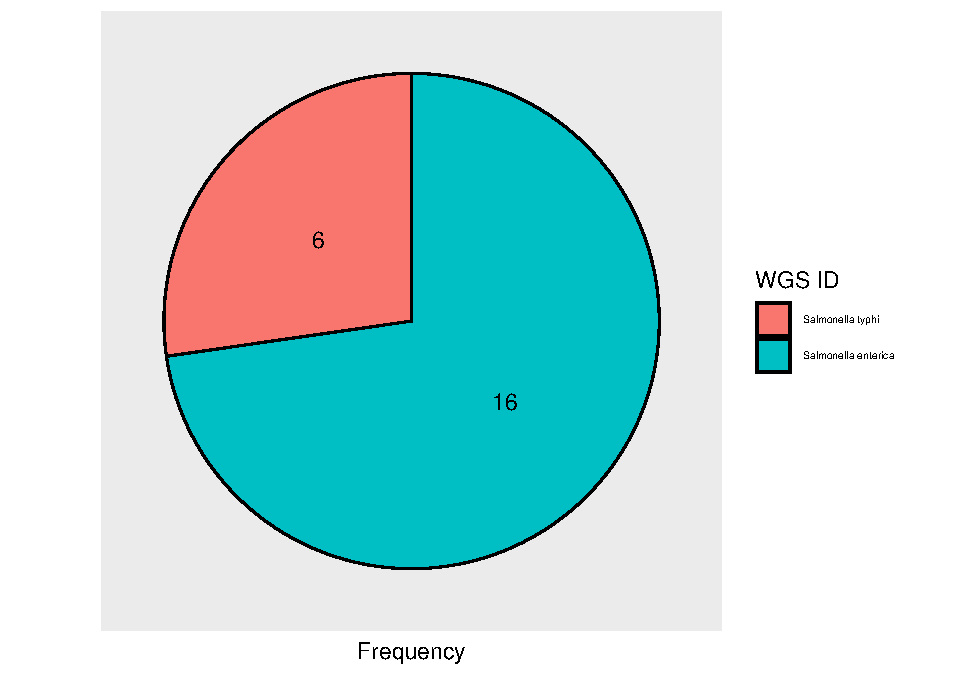
\includegraphics{qualifyr_report_2024-07-28_files/figure-latex/pie_chart-1.pdf}

\subsubsection{Result Classification}\label{result-classification}

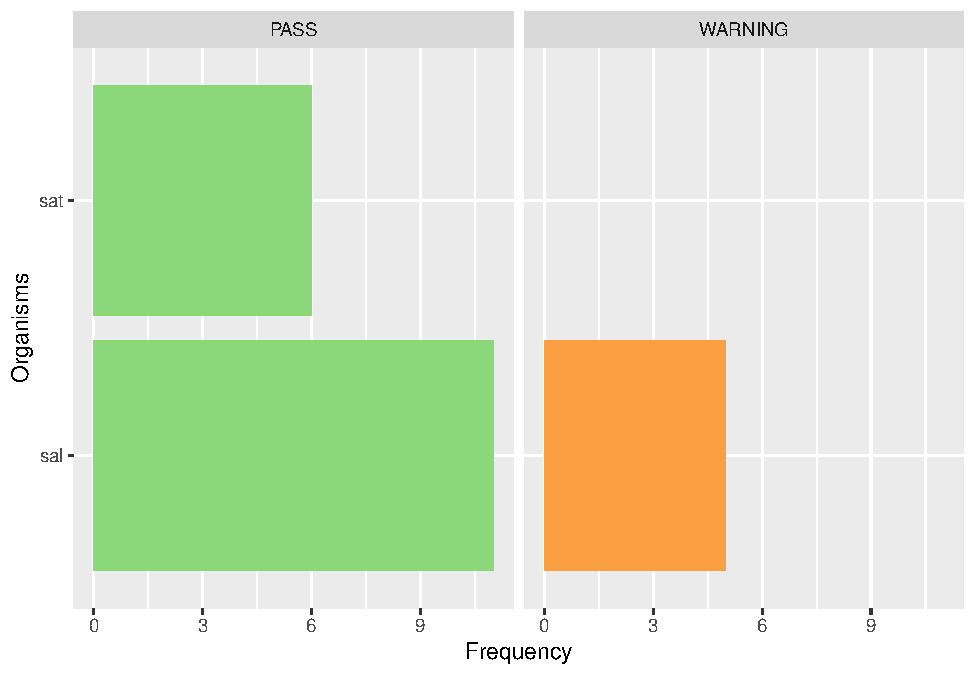
\includegraphics{qualifyr_report_2024-07-28_files/figure-latex/organism results-1.pdf}

\subsubsection{Number of contigs}\label{number-of-contigs}

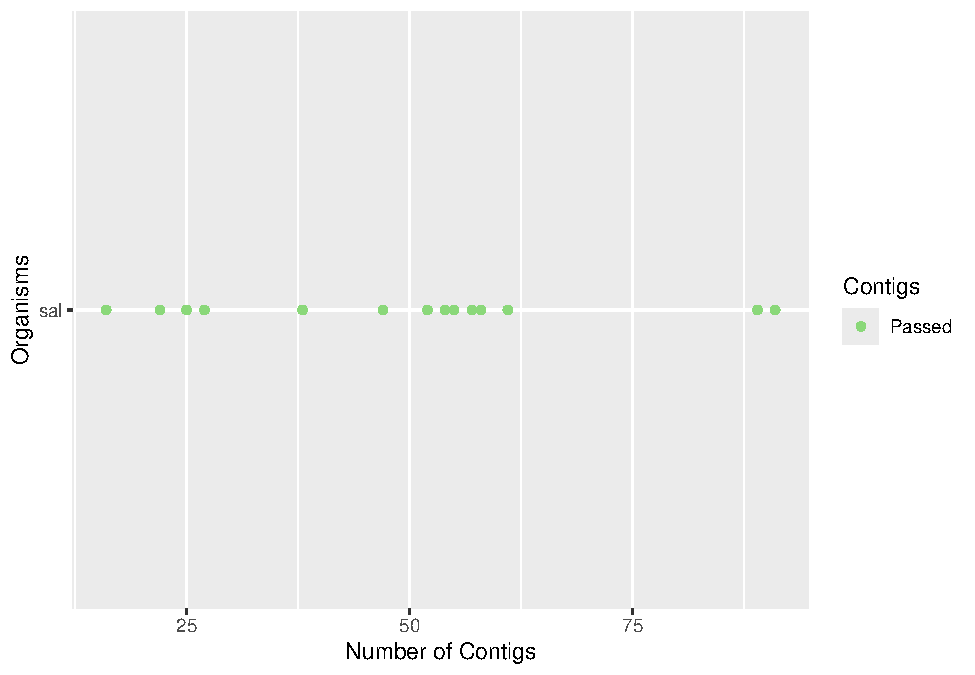
\includegraphics{qualifyr_report_2024-07-28_files/figure-latex/unnamed-chunk-3-1.pdf}

\subsubsection{N50 Value}\label{n50-value}

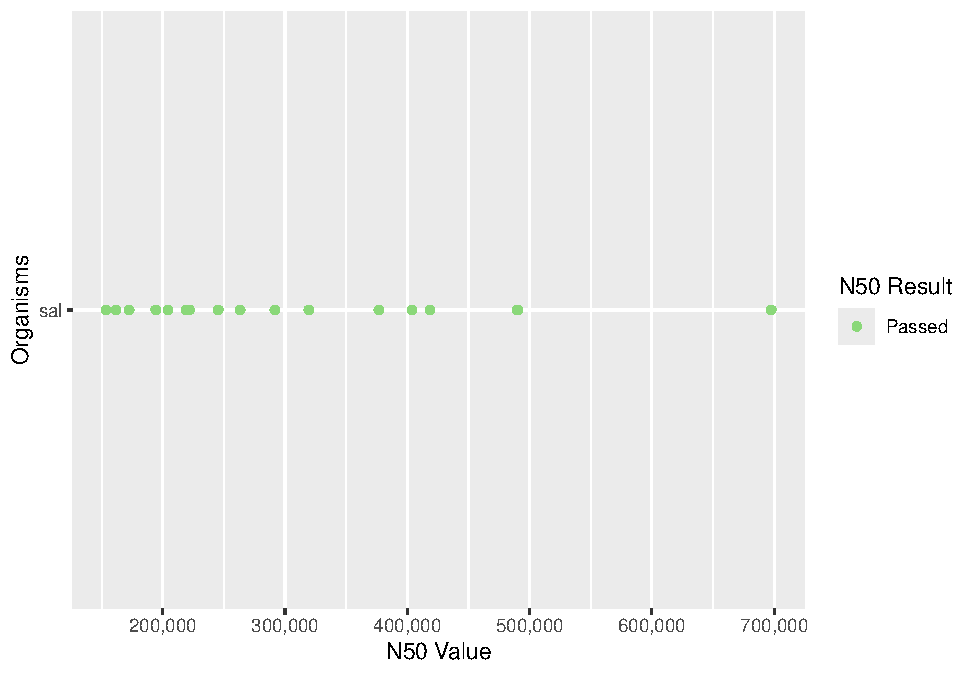
\includegraphics{qualifyr_report_2024-07-28_files/figure-latex/n50_result -1.pdf}

\subsubsection{Total Length}\label{total-length}

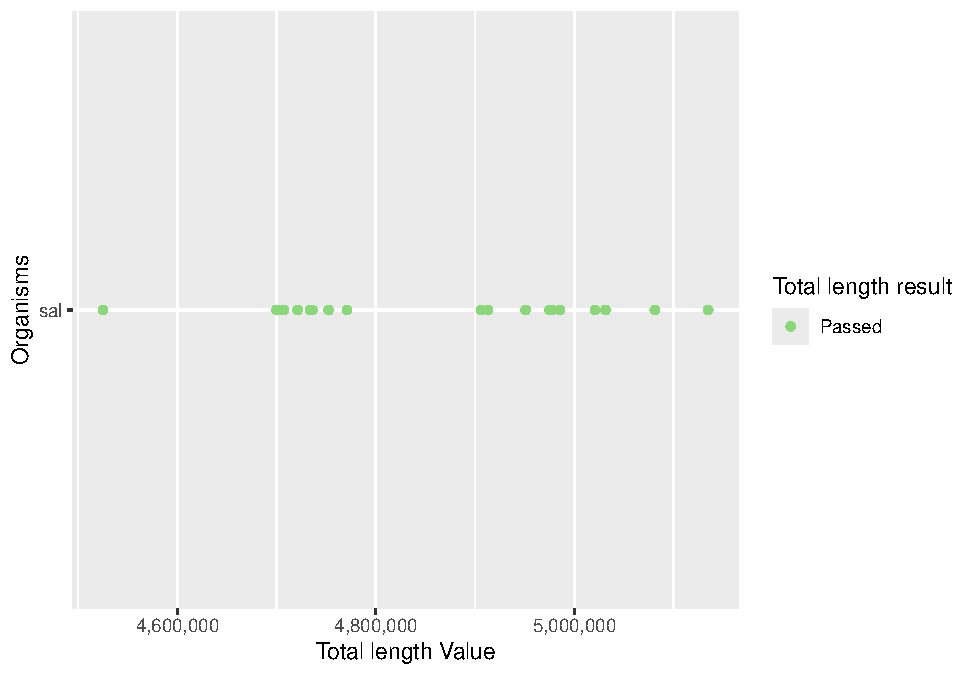
\includegraphics{qualifyr_report_2024-07-28_files/figure-latex/length_result -1.pdf}

\(\\\)

\subsubsection{RECOMMENDATION:}\label{recommendation}

\begin{longtable}[l]{>{\centering\arraybackslash}p{6cm}>{\centering\arraybackslash}p{4cm}>{\centering\arraybackslash}p{6cm}}
\toprule
\cellcolor[HTML]{D4D4D4}{\textbf{Sample ID}} & \cellcolor[HTML]{D4D4D4}{\textbf{Action}} & \cellcolor[HTML]{D4D4D4}{\textbf{Reason}}\\
\midrule
No futher action required for this batch &  & \\
\bottomrule
\end{longtable}

\subsubsection{MLST RESULTS}\label{mlst-results}

\begin{longtable}[l]{>{\centering\arraybackslash}p{3cm}>{\centering\arraybackslash}p{3cm}>{\centering\arraybackslash}p{1cm}>{\centering\arraybackslash}p{1cm}>{\centering\arraybackslash}p{1cm}>{\centering\arraybackslash}p{1cm}>{\centering\arraybackslash}p{1cm}>{\centering\arraybackslash}p{1cm}>{\centering\arraybackslash}p{1cm}c}
\toprule
\cellcolor[HTML]{D4D4D4}{\textbf{sample\_id}} & \cellcolor[HTML]{D4D4D4}{\textbf{species}} & \cellcolor[HTML]{D4D4D4}{\textbf{MLST}} & \cellcolor[HTML]{D4D4D4}{\textbf{aroC}} & \cellcolor[HTML]{D4D4D4}{\textbf{dnaN}} & \cellcolor[HTML]{D4D4D4}{\textbf{hemD}} & \cellcolor[HTML]{D4D4D4}{\textbf{hisD}} & \cellcolor[HTML]{D4D4D4}{\textbf{purE}} & \cellcolor[HTML]{D4D4D4}{\textbf{sucA}} & \cellcolor[HTML]{D4D4D4}{\textbf{thrA}}\\
\midrule
24ARS\_BGH0073 & Salmonella enterica & 34 & 10 & 19 & 12 & 9 & 5 & 9 & 2\\
24ARS\_BGH0098 & Salmonella enterica subsp. enterica serovar Infantis & 32 & 17 & 18 & 22 & 17 & 5 & 21 & 19\\
24ARS\_BGH0099 & Salmonella enterica subsp. enterica serovar Typhimurium & 313 & 10 & 7 & 12 & 9 & 112 & 9 & 2\\
24ARS\_BGH0100 & Salmonella enterica subsp. enterica serovar Infantis & 32 & 17 & 18 & 22 & 17 & 5 & 21 & 19\\
24ARS\_BRH0012 & Salmonella enterica subsp. enterica serovar Enteritidis & - & 5,638 & 2 & 3 & 7 & 6 & 6 & 11\\
\addlinespace
24ARS\_BRH0054 & Salmonella enterica subsp. enterica serovar Typhimurium & 19 & 10 & 7 & 12 & 9 & 5 & 9 & 2\\
24ARS\_BRH0068 & Salmonella enterica subsp. enterica serovar Typhi & 2 & 1 & 1 & 2 & 1 & 1 & 1 & 5\\
24ARS\_BRT0028 & Salmonella enterica subsp. enterica serovar Typhi & 1 & 1 & 1 & 1 & 1 & 1 & 1 & 5\\
24ARS\_BRT0041 & Salmonella enterica & - & 5,638 & 2 & 3 & 7 & 6 & 6 & 11\\
24ARS\_CMC0007 & Salmonella enterica subsp. enterica serovar Typhi & 1 & 1 & 1 & 1 & 1 & 1 & 1 & 5\\
\addlinespace
24ARS\_CRH0031 & Salmonella enterica & 437 & 13 & 12 & 63 & 16 & 13 & 16 & 4\\
24ARS\_CRH0049 & Salmonella enterica subsp. enterica serovar Typhimurium & 43 & 2 & 14 & 24 & 14 & 2 & 19 & 8\\
24ARS\_CVM0082 & Salmonella enterica subsp. enterica serovar Typhi & 1 & 1 & 1 & 1 & 1 & 1 & 1 & 5\\
24ARS\_DMC0100 & Salmonella enterica subsp. enterica serovar Weltevreden & 365 & 130 & 97 & 25 & 125 & 84 & 9 & 101\\
24ARS\_DMC0101 & Salmonella enterica subsp. enterica serovar Weltevreden & 365 & 130 & 97 & 25 & 125 & 84 & 9 & 101\\
\addlinespace
24ARS\_DMC0162 & Salmonella enterica & 1877 & 452 & 26 & 30 & 144 & 131 & 145 & 134\\
24ARS\_DMC0218 & Salmonella enterica subsp. enterica serovar Typhi & 1 & 1 & 1 & 1 & 1 & 1 & 1 & 5\\
24ARS\_DMC0291 & Salmonella enterica & 34 & 10 & 19 & 12 & 9 & 5 & 9 & 2\\
24ARS\_DMC0292 & Salmonella enterica subsp. enterica serovar Typhi & 2 & 1 & 1 & 2 & 1 & 1 & 1 & 5\\
24ARS\_GMH0033 & Salmonella enterica & - & 5,638 & 2 & 3 & 7 & 6 & 6 & 11\\
\addlinespace
24ARS\_JLM0046 & Salmonella enterica subsp. enterica serovar Infantis & - & 17 & 18 & 22 & 17 & \textasciitilde{}5 & 21 & 19\\
\bottomrule
\end{longtable}
\vspace{1em}

\subsubsection{MLST RESULTS SUMMARY:}\label{mlst-results-summary}

\begin{longtable}[l]{ll}
\toprule
\cellcolor[HTML]{D4D4D4}{\textbf{wgs\_id}} & \cellcolor[HTML]{D4D4D4}{\textbf{mlst\_count}}\\
\midrule
Salmonella enterica & - (n= 2 ), 1877 (n= 1 ), 34 (n= 2 ), 437 (n= 1 )\\
Salmonella enterica subsp. enterica serovar Enteritidis & - (n= 1 )\\
Salmonella enterica subsp. enterica serovar Infantis & - (n= 1 ), 32 (n= 2 )\\
Salmonella enterica subsp. enterica serovar Typhi & 1 (n= 4 ), 2 (n= 2 )\\
Salmonella enterica subsp. enterica serovar Typhimurium & 19 (n= 1 ), 313 (n= 1 ), 43 (n= 1 )\\
\addlinespace
Salmonella enterica subsp. enterica serovar Weltevreden & 365 (n= 2 )\\
\bottomrule
\end{longtable}

\newpage
\begin{landscape}

\subsubsection{AMR PREDICTION RESULTS}\label{amr-prediction-results}

\begin{table}[H]
\centering
\resizebox{\ifdim\width>\linewidth\linewidth\else\width\fi}{!}{
\begin{tabular}{c>{\centering\arraybackslash}p{3cm}>{\centering\arraybackslash}p{3cm}>{\centering\arraybackslash}p{3cm}>{\centering\arraybackslash}p{3cm}>{\centering\arraybackslash}p{3cm}>{\centering\arraybackslash}p{3cm}>{\centering\arraybackslash}p{3cm}>{\centering\arraybackslash}p{3cm}>{\centering\arraybackslash}p{3cm}>{\centering\arraybackslash}p{3cm}>{\centering\arraybackslash}p{3cm}>{\centering\arraybackslash}p{3cm}>{\centering\arraybackslash}p{3cm}>{\centering\arraybackslash}p{3cm}>{\centering\arraybackslash}p{3cm}>{\centering\arraybackslash}p{3cm}>{\centering\arraybackslash}p{3cm}>{\centering\arraybackslash}p{3cm}>{\centering\arraybackslash}p{3cm}>{\centering\arraybackslash}p{3cm}>{\centering\arraybackslash}p{3cm}>{\centering\arraybackslash}p{3cm}>{\centering\arraybackslash}p{3cm}>{\centering\arraybackslash}p{3cm}>{\centering\arraybackslash}p{3cm}}
\toprule
\multicolumn{26}{l}{\textbf{\textit{Salmonella enterica}}} \\
\cmidrule(l{3pt}r{3pt}){1-26}
\cellcolor[HTML]{D4D4D4}{\textbf{sample\_id}} & \cellcolor[HTML]{D4D4D4}{\textbf{AMR APRAMYCIN/ GENTAMICIN/ TOBRAMYCIN}} & \cellcolor[HTML]{D4D4D4}{\textbf{AMR BETA-LACTAM}} & \cellcolor[HTML]{D4D4D4}{\textbf{AMR CEPHALOSPORIN}} & \cellcolor[HTML]{D4D4D4}{\textbf{AMR CHLORAMPHENICOL/ FLORFENICOL}} & \cellcolor[HTML]{D4D4D4}{\textbf{AMR EFFLUX}} & \cellcolor[HTML]{D4D4D4}{\textbf{AMR FOSFOMYCIN}} & \cellcolor[HTML]{D4D4D4}{\textbf{AMR HYGROMYCIN}} & \cellcolor[HTML]{D4D4D4}{\textbf{AMR KANAMYCIN}} & \cellcolor[HTML]{D4D4D4}{\textbf{AMR STREPTOMYCIN}} & \cellcolor[HTML]{D4D4D4}{\textbf{AMR SULFONAMIDE}} & \cellcolor[HTML]{D4D4D4}{\textbf{AMR TETRACYCLINE}} & \cellcolor[HTML]{D4D4D4}{\textbf{AMR TRIMETHOPRIM}} & \cellcolor[HTML]{D4D4D4}{\textbf{STRESS ARSENATE}} & \cellcolor[HTML]{D4D4D4}{\textbf{STRESS ARSENIC}} & \cellcolor[HTML]{D4D4D4}{\textbf{STRESS ARSENITE}} & \cellcolor[HTML]{D4D4D4}{\textbf{STRESS COPPER}} & \cellcolor[HTML]{D4D4D4}{\textbf{STRESS COPPER/ GOLD}} & \cellcolor[HTML]{D4D4D4}{\textbf{STRESS COPPER/ SILVER}} & \cellcolor[HTML]{D4D4D4}{\textbf{STRESS GOLD}} & \cellcolor[HTML]{D4D4D4}{\textbf{STRESS MERCURY}} & \cellcolor[HTML]{D4D4D4}{\textbf{STRESS NA}} & \cellcolor[HTML]{D4D4D4}{\textbf{STRESS ORGANOMERCURY}} & \cellcolor[HTML]{D4D4D4}{\textbf{STRESS QUATERNARY AMMONIUM}} & \cellcolor[HTML]{D4D4D4}{\textbf{STRESS SILVER}} & \cellcolor[HTML]{D4D4D4}{\textbf{VIRULENCE NA}}\\
\midrule
24ARS\_BGH0073 & NA & blaTEM-1 & NA & NA & mdsA, mdsB & NA & NA & NA & aph(6)-Id, aph(3'')-Ib & sul2 & tet(B) & NA & arsC & arsR & arsB, arsA, arsD & pcoS, pcoR, pcoD, pcoC, pcoA & golT & silA, silB, silF, silC, silR, silS & golS & merP, merT, merR & fieF & merC & NA & silP, silE & iroC, iroB, sinH, sodC1\\
24ARS\_BGH0098 & aac(3)-IVa & NA & blaCTX-M-65 & floR & mdsA, mdsB & NA & aph(4)-Ia & NA & aadA1 & sul1 & tet(A) & dfrA14 & NA & arsR & NA & NA & golT & NA & golS & merP, merT, merR & fieF & merC & qacEdelta1 & NA & iroB, iroC, sinH, ybtP, ybtQ\\
24ARS\_BGH0099 & NA & NA & NA & NA & mdsA, mdsB & NA & NA & NA & NA & NA & NA & NA & NA & NA & NA & NA & golT & NA & golS & NA & fieF & NA & NA & NA & iroB, iroC, sodC1, sinH\\
24ARS\_BGH0100 & aac(3)-IVa & NA & blaCTX-M-65 & floR & mdsA, mdsB & NA & aph(4)-Ia & NA & aadA1 & sul1 & tet(A) & dfrA14 & NA & arsR & NA & NA & golT & NA & golS & merP, merT, merR & fieF & merC & qacEdelta1 & NA & sinH, ybtP, ybtQ, iroB, iroC\\
24ARS\_BRH0012 & NA & NA & NA & NA & mdsA, mdsB & NA & NA & NA & NA & NA & NA & NA & NA & NA & NA & NA & golT & NA & golS & NA & fieF & NA & NA & NA & sodC1, iroB, iroC, sinH\\
\addlinespace
24ARS\_BRH0054 & NA & NA & NA & NA & mdsA, mdsB & NA & NA & NA & aph(6)-Id, aph(3'')-Ib & sul2 & tet(A) & NA & NA & NA & NA & NA & golT & NA & golS & NA & fieF & NA & NA & NA & sinH, iroB, iroC, sodC1\\
24ARS\_BRH0068 & NA & NA & NA & NA & NA & NA & NA & NA & NA & NA & NA & NA & NA & NA & NA & NA & NA & NA & NA & NA & fieF & NA & NA & NA & sinH, iroB, iroC, cdtB\\
24ARS\_BRT0028 & NA & NA & NA & NA & NA & NA & NA & NA & NA & NA & NA & NA & NA & NA & NA & NA & NA & NA & NA & NA & fieF & NA & NA & NA & iroB, iroC, sinH, cdtB\\
24ARS\_BRT0041 & NA & blaTEM-1 & NA & NA & mdsA, mdsB & NA & NA & NA & aph(6)-Id, aph(3'')-Ib & sul2 & NA & NA & NA & NA & NA & NA & golT & NA & golS & NA & fieF & NA & NA & NA & sodC1, iroC, iroB, sinH\\
24ARS\_CMC0007 & NA & NA & NA & NA & NA & NA & NA & NA & NA & NA & NA & NA & NA & NA & NA & NA & NA & NA & NA & NA & fieF & NA & NA & NA & sinH, iroC, cdtB\\
\addlinespace
24ARS\_CRH0031 & NA & NA & NA & NA & mdsA, mdsB & NA & NA & NA & NA & NA & NA & NA & NA & NA & NA & NA & golT & NA & golS & NA & fieF & NA & NA & NA & cdtB, iroC, iroB, sinH\\
24ARS\_CRH0049 & NA & NA & NA & NA & mdsA, mdsB & NA & NA & NA & NA & NA & NA & NA & NA & NA & NA & NA & golT & NA & golS & NA & fieF & NA & NA & NA & sinH, iroB, iroC\\
24ARS\_CVM0082 & NA & NA & NA & NA & NA & NA & NA & NA & NA & NA & NA & NA & NA & NA & NA & NA & NA & NA & NA & NA & fieF & NA & NA & NA & iroB, iroC, sinH, cdtB\\
24ARS\_DMC0100 & NA & NA & NA & NA & mdsA, mdsB & NA & NA & NA & NA & NA & NA & NA & NA & NA & NA & NA & golT & NA & golS & NA & fieF & NA & NA & NA & iroB, iroC, sinH, sodC1\\
24ARS\_DMC0101 & NA & NA & NA & NA & mdsA, mdsB & NA & NA & NA & NA & NA & NA & NA & NA & NA & NA & NA & golT & NA & golS & NA & fieF & NA & NA & NA & sinH, iroB, iroC, sodC1\\
\addlinespace
24ARS\_DMC0162 & NA & NA & NA & NA & NA & NA & NA & NA & NA & NA & NA & NA & NA & NA & NA & NA & NA & NA & NA & NA & fieF & NA & NA & NA & ybtQ, ybtP, cdtB, iutA, iucA, mchF, iroB, iroC\\
24ARS\_DMC0218 & NA & NA & NA & NA & NA & NA & NA & NA & NA & NA & NA & NA & NA & NA & NA & NA & NA & NA & NA & NA & fieF & NA & NA & NA & iroB, iroC, sinH, cdtB\\
24ARS\_DMC0291 & NA & blaTEM-1 & NA & NA & mdsA, mdsB & NA & NA & NA & NA & NA & tet(B) & NA & arsC & arsR & arsB, arsA, arsD & pcoS, pcoR, pcoD, pcoC, pcoA & golT & silA, silB, silF, silC, silR, silS & golS & NA & fieF & NA & NA & silP, silE & iroC, iroB, sinH, sodC1\\
24ARS\_DMC0292 & NA & NA & NA & NA & NA & NA & NA & NA & NA & NA & NA & NA & NA & NA & NA & NA & NA & NA & NA & NA & fieF & NA & NA & NA & iroB, iroC, sinH, cdtB\\
24ARS\_GMH0033 & NA & blaTEM-1 & NA & NA & mdsA, mdsB & NA & NA & NA & aadA5 & NA & NA & dfrA17 & NA & NA & NA & NA & golT & NA & golS & merR, merT, merP & fieF & merC & qacEdelta1 & NA & sodC1, sinH, iroB, iroC\\
\addlinespace
24ARS\_JLM0046 & aac(3)-IVa & NA & blaCTX-M-65 & floR & mdsA, mdsB & fosA3 & aph(4)-Ia & aph(3')-Ia & aadA1 & sul1 & tet(A) & dfrA14 & NA & arsR & NA & NA & golT & NA & golS & merP, merT, merR & fieF & merC & qacEdelta1 & NA & sinH, ybtP, ybtQ, iroB, iroC\\
\bottomrule
\end{tabular}}
\end{table}
\vspace{1em}

\end{landscape}

\end{document}
